\documentclass{scrartcl} % scrartcl of scrreprt
% Include all project wide packages here.
\usepackage{fullpage}
\usepackage{polyglossia}
\setmainlanguage{dutch}
\usepackage{csquotes}
\usepackage{graphicx}
\usepackage{epstopdf}
\usepackage{pdfpages}
\usepackage{caption}
\usepackage[list=true]{subcaption}
\usepackage{float}
%\usepackage{mathtools}
\usepackage{standalone}
\usepackage{import}
\usepackage{tocloft}
\usepackage{wrapfig}
\usepackage{authblk}
\usepackage{array}
\usepackage{booktabs}
\usepackage[toc,page,title,titletoc]{appendix}
\usepackage{xunicode}
\usepackage{amsmath}
\usepackage{fontspec}
\usepackage{unicode-math}
\usepackage[
    backend=bibtexu,
	texencoding=utf8,
bibencoding=utf8,
    style=ieee,
    sortlocale=nl_NL,
    language=auto
]{biblatex}
\usepackage{listings}
\newcommand{\includecode}[3][c]{\lstinputlisting[caption=#2, escapechar=, style=#1]{#3}}
\newcommand{\superscript}[1]{\ensuremath{^{\textrm{#1}}}}
\newcommand{\subscript}[1]{\ensuremath{_{\textrm{#1}}}}


\newcommand{\chapternumber}{\thechapter}
\renewcommand{\appendixname}{Bijlage}
\renewcommand{\appendixtocname}{Bijlagen}
\renewcommand{\appendixpagename}{Bijlagen}

\usepackage[hidelinks]{hyperref} %<--------ALTIJD ALS LAATSTE

\renewcommand{\familydefault}{\sfdefault}

\setmainfont[Ligatures=TeX]{Myriad Pro}
\setmathfont{Asana Math}
\setmonofont{Lucida Console}

\usepackage{titlesec, blindtext, color}
\definecolor{gray75}{gray}{0.75}
\newcommand{\hsp}{\hspace{20pt}}
\titleformat{\chapter}[hang]{\Huge\bfseries}{\chapternumber\hsp\textcolor{gray75}{|}\hsp}{0pt}{\Huge\bfseries}
\renewcommand{\familydefault}{\sfdefault}
\renewcommand{\arraystretch}{1.2}
\setlength\parindent{0pt}

%For code listings
\definecolor{black}{rgb}{0,0,0}
\definecolor{browntags}{rgb}{0.65,0.1,0.1}
\definecolor{bluestrings}{rgb}{0,0,1}
\definecolor{graycomments}{rgb}{0.4,0.4,0.4}
\definecolor{redkeywords}{rgb}{1,0,0}
\definecolor{bluekeywords}{rgb}{0.13,0.13,0.8}
\definecolor{greencomments}{rgb}{0,0.5,0}
\definecolor{redstrings}{rgb}{0.9,0,0}
\definecolor{purpleidentifiers}{rgb}{0.01,0,0.01}


\lstdefinestyle{csharp}{
language=[Sharp]C,
showspaces=false,
showtabs=false,
breaklines=true,
showstringspaces=false,
breakatwhitespace=true,
escapeinside={(*@}{@*)},
columns=fullflexible,
commentstyle=\color{greencomments},
keywordstyle=\color{bluekeywords}\bfseries,
stringstyle=\color{redstrings},
identifierstyle=\color{purpleidentifiers},
basicstyle=\ttfamily\small}

\lstdefinestyle{c}{
language=C,
showspaces=false,
showtabs=false,
breaklines=true,
showstringspaces=false,
breakatwhitespace=true,
escapeinside={(*@}{@*)},
columns=fullflexible,
commentstyle=\color{greencomments},
keywordstyle=\color{bluekeywords}\bfseries,
stringstyle=\color{bluestrings},
identifierstyle=\color{purpleidentifiers}
}

\lstdefinestyle{vhdl}{
language=VHDL,
showspaces=false,
showtabs=false,
breaklines=true,
showstringspaces=false,
breakatwhitespace=true,
escapeinside={(*@}{@*)},
columns=fullflexible,
commentstyle=\color{greencomments},
keywordstyle=\color{bluekeywords}\bfseries,
stringstyle=\color{redstrings},
identifierstyle=\color{purpleidentifiers}
}

\lstdefinestyle{xaml}{
language=XML,
showspaces=false,
showtabs=false,
breaklines=true,
showstringspaces=false,
breakatwhitespace=true,
escapeinside={(*@}{@*)},
columns=fullflexible,
commentstyle=\color{greencomments},
keywordstyle=\color{redkeywords},
stringstyle=\color{bluestrings},
tagstyle=\color{browntags},
morestring=[b]",
  morecomment=[s]{<?}{?>},
  morekeywords={xmlns,version,typex:AsyncRecords,x:Arguments,x:Boolean,x:Byte,x:Char,x:Class,x:ClassAttributes,x:ClassModifier,x:Code,x:ConnectionId,x:Decimal,x:Double,x:FactoryMethod,x:FieldModifier,x:Int16,x:Int32,x:Int64,x:Key,x:Members,x:Name,x:Object,x:Property,x:Shared,x:Single,x:String,x:Subclass,x:SynchronousMode,x:TimeSpan,x:TypeArguments,x:Uid,x:Uri,x:XData,Grid.Column,Grid.ColumnSpan,Click,ClipToBounds,Content,DropDownOpened,FontSize,Foreground,Header,Height,HorizontalAlignment,HorizontalContentAlignment,IsCancel,IsDefault,IsEnabled,IsSelected,Margin,MinHeight,MinWidth,Padding,SnapsToDevicePixels,Target,TextWrapping,Title,VerticalAlignment,VerticalContentAlignment,Width,WindowStartupLocation,Binding,Mode,OneWay,xmlns:x}
}

%defaults
\lstset{
basicstyle=\ttfamily\small,
extendedchars=false,
numbers=left,
numberstyle=\ttfamily\tiny,
stepnumber=1,
tabsize=4,
numbersep=5pt
}
\addbibresource{../../library/bibliography.bib}

\author{Alex Janssen}
\title{EPO3: Eindrapport - Draw-sprite}

\begin{document}
\section{Draw-sprite}
\label{sec:draw-sprite}

%Specs
\subsection{Specificaties}
Draw\_sprite is een module die coordinaten van pixels uit kan lezen uit het RAM en dat vervolgens in de screenbuffer kan plaatsen zodat het mogelijk is om ingewikkeldere afbeeldingen te kunnen tekenen. Bij de ingang worden de coordinaten aangegeven van waar de sprite moet worden getekend, en de startlocatie van de sprite in het RAM samen met de lengte en de breedte ervan.

\begin{figure}[H]
	\centering
	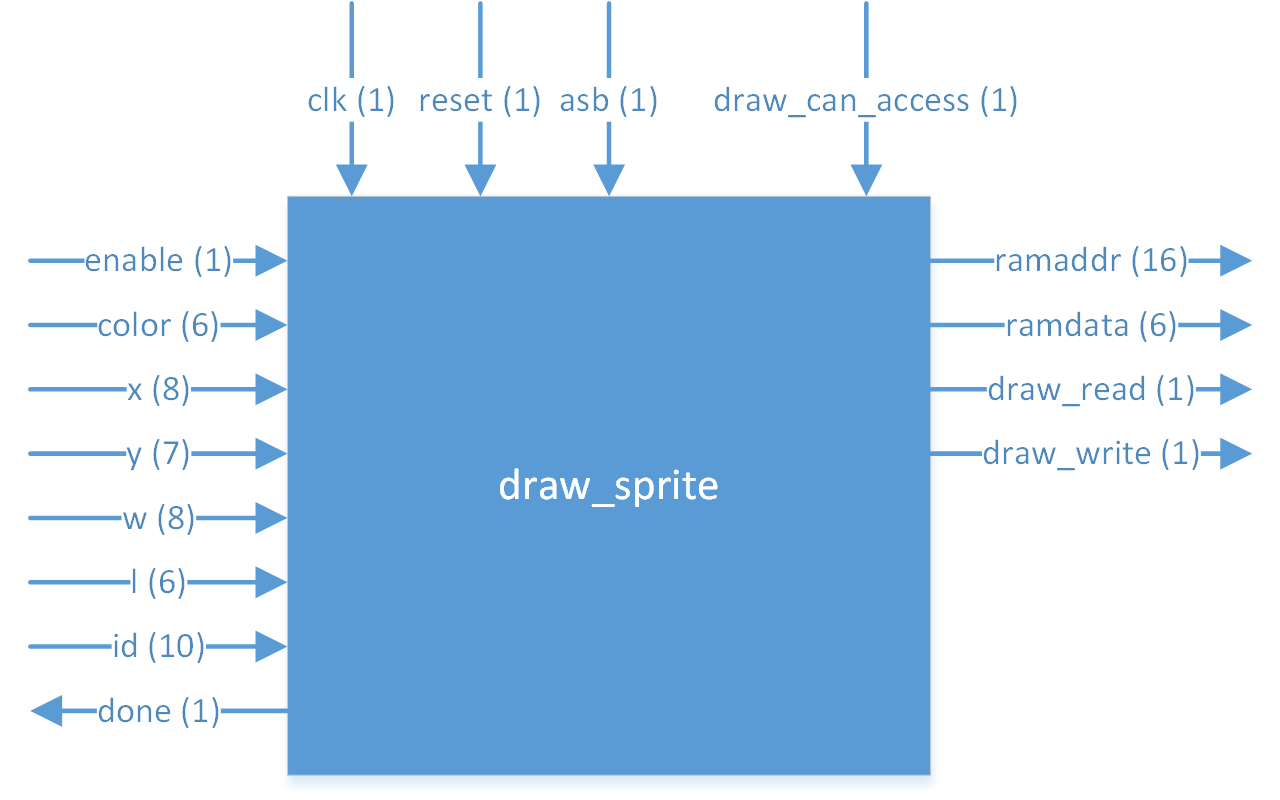
\includegraphics[width=0.75\textwidth]{resource/draw_sprite.png}
	\caption{Een blokschema van draw\_sprite, met de namen van de gebruikte in- en uitgangen en tussen haakjes het aantal bits}
	\label{fig:draw-sprite-schema}
\end{figure}

%Ontwerp en implementatie
\subsection{Ontwerp en implementatie}
Deze module wordt pas aangeroepen zodra enable 1 is en mag net als alle andere modules lezen uit het RAM en schrijven wanneer draw\_can\_access gelijk is aan `1'. Vervolgens zal deze met behulp van de startlocatie in het RAM waar de sprite staat en de breedte en hoogte ervan de pixels een voor 1 uitlezen en wegschrijven in de screenbuffer waarna het wordt getekend op het scherm door de met behulp van de VGA controller.

%VHDL simulatie
\subsection{VHDL simulatie}
Voor de VHDL simulatie is ModelSim gebruikt, waarvoor een testbench is geschreven. In de testbench wordt eerst enable laag gehouden, waarbij hij inderdaad niets uitvoert wat er ook op de ingangen komt te staan.\\
\begin{figure}[H]
	\centering
	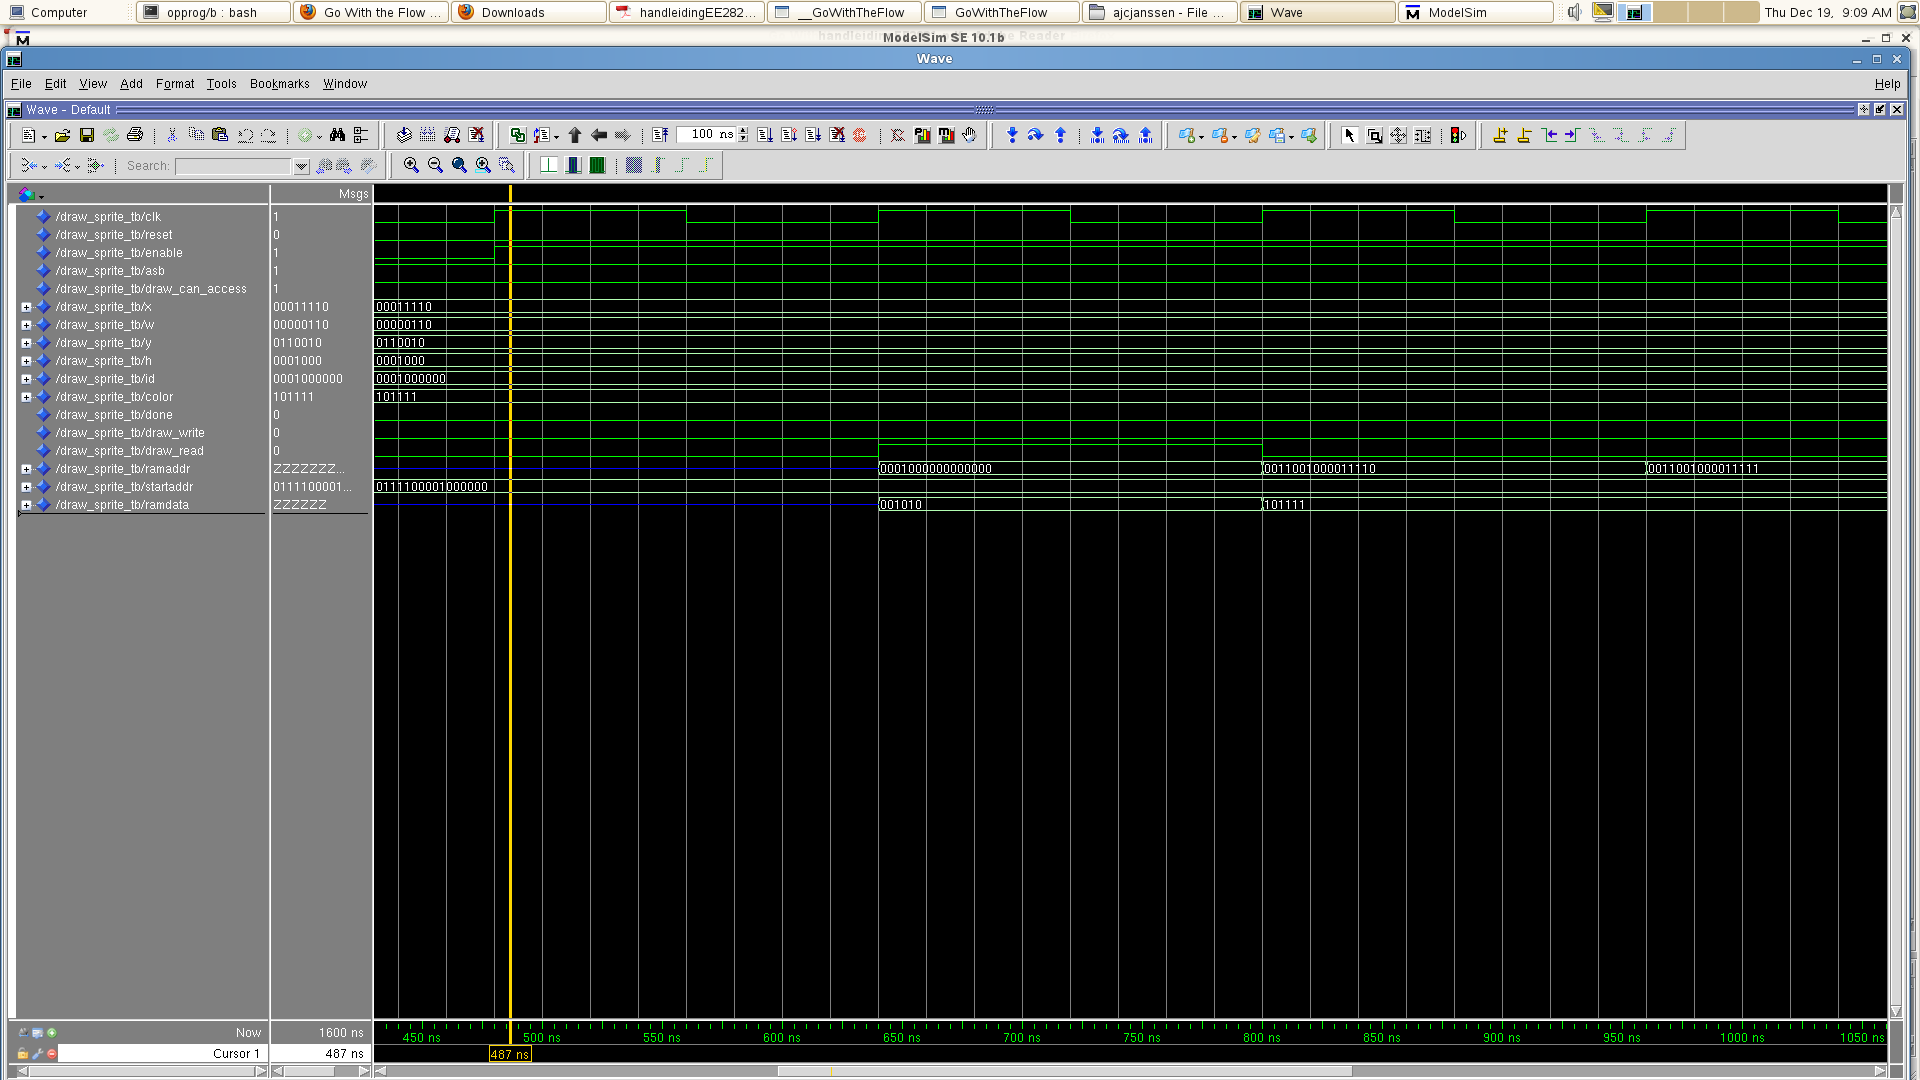
\includegraphics[width=0.75\textwidth]{resource/draw_sprite_simulate.png}
	\caption{De simulatie van draw sprite, nadat enable op `1' is gegaan}
	\label{fig:draw-sprite-simulatie}
\end{figure}
Vervolgens gaat afhankelijk van het startadres de draw sprite module de verschillende geheugenlocaties af en leest daar de kleur van uit. Dit blijft hij zodanig herhalen totdat hij bij de laatste aangegeven locatie komt die aangegeven zijn door middel van een breedte en hoogte, waarna done `1' wordt

%Synthese
\subsection{Synthese en lay-out}
De draw-sprite module heeft weinig te maken met optel en shiftoperaties, waardoor er bij de synthese relatief weinig transistoren zijn gebruikt. Er is voor het behalen van een hogere efficiëntie nog gewerkt met het handmatig placen van rows en blokken, wat heeft gezorgd voor een uiteindelijk resultaat met 9900 transistoren waarvan er 3847 daadwerkelijk gebruikt zijn. De uiteindelijke efficiëntie van deze module bedraagt dan 38.86\%.

%Switchlevel test
\subsection{Switch-level simulatie}
Het circuit en de layout zijn beide gesimuleerd met SLS en vergeleken met de testbench van ModelSim. Dit gaf het verwachte resultaat en dus is deze als correct te beschouwen.

%Conclusie
\subsection{Conclusie}
De module werkt naar behoren, en vergroot onze mogelijkheden bij het maken van spellen enorm. De module gebruikt uiteindelijk 9900 transistoren dus neemt grofweg een achste deel in van onze chip. Aangezien de simulaties overeenkomen met onze verwachtingen en de module succesvol gesynthetiseerd is mogen we concluderen dat hij correct functioneerd.

\end{document}
